\section{Shapes of an FSM Language}
\label{sec:eval}

%\begin{figure}
%	\centering
%	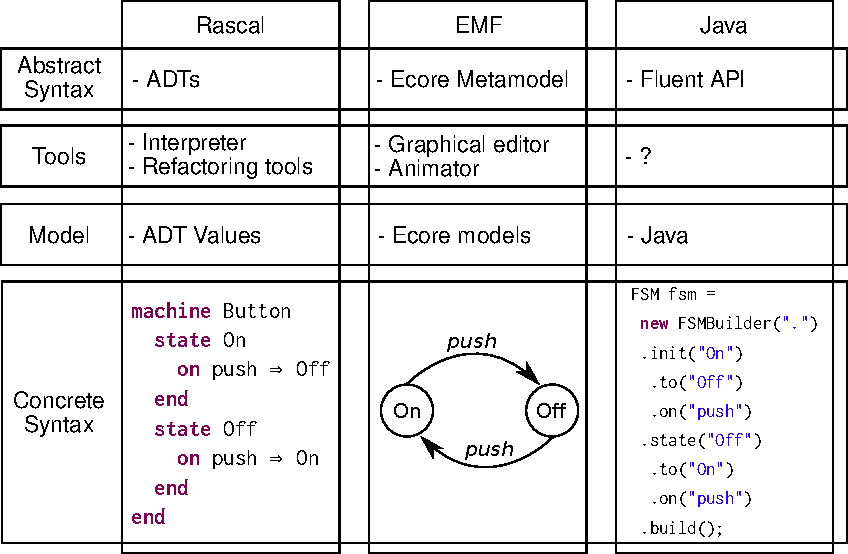
\includegraphics[width=\columnwidth]{figures/concepts-instantiated}
%	\caption{\dots}
%	\label{fig:concepts-instantiated}
%\end{figure}

\begin{figure}[bt]
	\centering
	\begin{subfigure}[b]{.3\columnwidth}
		\begin{lstlisting}[label=lst:fsm-adt, language=Rascal, numbers=none, xleftmargin=0pt, tabsize=1]
data Machine(Id uid) =
	Machine(str name,
		list[State] states,
		Ref[State] initial);

data State(Id uid) =
	State(str name,
		list[Trans] trans);

data Trans(Id uid) =
	Trans(str event,
		Ref[State] target);
		\end{lstlisting}
		\caption{Rascal ADT}
	\end{subfigure}
	\vrule
	\enskip
	\begin{subfigure}[b]{.26\columnwidth}
		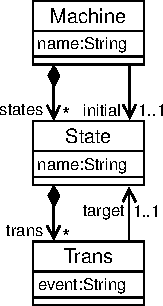
\includegraphics[width=\textwidth]{figures/fsm-mm}
		\caption{Ecore MM}
	\end{subfigure}
	\enskip
	\vrule
	\enskip
	\begin{subfigure}[b]{.35\columnwidth}
		\begin{lstlisting}[label=lst:fsm-api, language=Java, numbers=none, xleftmargin=0pt, tabsize=1]
class Fsm {
	Fsm(String name);
	State init(String name);
	State state(String name);
	Fsm end();
}
class State {
	State state(String name);
	Trans tgt(String name);
	Fsm end();
}
class Trans {
	Trans tgt(String name);
	State on(String event);
	Fsm end();
}
		\end{lstlisting}
		\caption{Java API}
	\end{subfigure}
	\caption{Three shapes of an FSM language}
\end{figure}


We try our approach on tree implementations of the Finite State Machine language.
We implemented manually the FSM language in Rascal, Ecore and as a fluent Java API.
Rascal is providing a textual editor, Ecore provides a graphical editor and we used the Java editor for the fluent API.

In our manipulation we were able to edit an incarnation of a model in one editor and see the change applied in others editors.
By using an editor, we were able to benefit of the result of the tooling in others incarnations, i.e., using the content assist of Java is also updating other editors.
We also observe some de-synchronization happening due to the partially unaligned FSM implementation in Java.

The Java fluent API shape tends to break more easily the synchronization of their incarnations of models than the other shapes.
Indeed this shape of FSM language is an embedded language and has to rely on the host language for both the tooling and the expressiveness.
In the case of Java as host language, the validation service provided by the editor has no knowledge about the FSM language.
It makes harder for the user to detect mistakes such as typo. The FSM model can be in unnoticed dirty state and this can lead to the production of dirty Patches.
In the opposite the incarnation of the model can receive inapplicable Patches in this technological space.

Another example in the Java TS of problem encountered is the constraints from the host language.
We choose to represent a State by the method state() or by the method initial().
As the initial State is unique, we enforce its declaration as the first method invocation in the FSM.
This solution solve the uniqueness but enforce the first state to be initial.
Thus with this representation of FSM, receiving a Patch telling to reference the second state of an FSM as the initial state is not possible due to the expressiveness of the API and this result in the desynchronization of the incarnation of the model.

The inconsistency of the incarnations of a model happen when one of them produce a dirty Patch or when one of them can't apply a Patch.
